% Options for packages loaded elsewhere
\PassOptionsToPackage{unicode}{hyperref}
\PassOptionsToPackage{hyphens}{url}
%
\documentclass[
  ignorenonframetext,
]{beamer}
\usepackage{pgfpages}
\setbeamertemplate{caption}[numbered]
\setbeamertemplate{caption label separator}{: }
\setbeamercolor{caption name}{fg=normal text.fg}
\beamertemplatenavigationsymbolsempty
% Prevent slide breaks in the middle of a paragraph
\widowpenalties 1 10000
\raggedbottom
\setbeamertemplate{part page}{
  \centering
  \begin{beamercolorbox}[sep=16pt,center]{part title}
    \usebeamerfont{part title}\insertpart\par
  \end{beamercolorbox}
}
\setbeamertemplate{section page}{
  \centering
  \begin{beamercolorbox}[sep=12pt,center]{section title}
    \usebeamerfont{section title}\insertsection\par
  \end{beamercolorbox}
}
\setbeamertemplate{subsection page}{
  \centering
  \begin{beamercolorbox}[sep=8pt,center]{subsection title}
    \usebeamerfont{subsection title}\insertsubsection\par
  \end{beamercolorbox}
}
\AtBeginPart{
  \frame{\partpage}
}
\AtBeginSection{
  \ifbibliography
  \else
    \frame{\sectionpage}
  \fi
}
\AtBeginSubsection{
  \frame{\subsectionpage}
}

\usepackage{amsmath,amssymb}
\usepackage{iftex}
\ifPDFTeX
  \usepackage[T1]{fontenc}
  \usepackage[utf8]{inputenc}
  \usepackage{textcomp} % provide euro and other symbols
\else % if luatex or xetex
  \usepackage{unicode-math}
  \defaultfontfeatures{Scale=MatchLowercase}
  \defaultfontfeatures[\rmfamily]{Ligatures=TeX,Scale=1}
\fi
\usepackage{lmodern}
\ifPDFTeX\else  
    % xetex/luatex font selection
\fi
% Use upquote if available, for straight quotes in verbatim environments
\IfFileExists{upquote.sty}{\usepackage{upquote}}{}
\IfFileExists{microtype.sty}{% use microtype if available
  \usepackage[]{microtype}
  \UseMicrotypeSet[protrusion]{basicmath} % disable protrusion for tt fonts
}{}
\makeatletter
\@ifundefined{KOMAClassName}{% if non-KOMA class
  \IfFileExists{parskip.sty}{%
    \usepackage{parskip}
  }{% else
    \setlength{\parindent}{0pt}
    \setlength{\parskip}{6pt plus 2pt minus 1pt}}
}{% if KOMA class
  \KOMAoptions{parskip=half}}
\makeatother
\usepackage{xcolor}
\newif\ifbibliography
\setlength{\emergencystretch}{3em} % prevent overfull lines
\setcounter{secnumdepth}{-\maxdimen} % remove section numbering

\usepackage{color}
\usepackage{fancyvrb}
\newcommand{\VerbBar}{|}
\newcommand{\VERB}{\Verb[commandchars=\\\{\}]}
\DefineVerbatimEnvironment{Highlighting}{Verbatim}{commandchars=\\\{\}}
% Add ',fontsize=\small' for more characters per line
\usepackage{framed}
\definecolor{shadecolor}{RGB}{241,243,245}
\newenvironment{Shaded}{\begin{snugshade}}{\end{snugshade}}
\newcommand{\AlertTok}[1]{\textcolor[rgb]{0.68,0.00,0.00}{#1}}
\newcommand{\AnnotationTok}[1]{\textcolor[rgb]{0.37,0.37,0.37}{#1}}
\newcommand{\AttributeTok}[1]{\textcolor[rgb]{0.40,0.45,0.13}{#1}}
\newcommand{\BaseNTok}[1]{\textcolor[rgb]{0.68,0.00,0.00}{#1}}
\newcommand{\BuiltInTok}[1]{\textcolor[rgb]{0.00,0.23,0.31}{#1}}
\newcommand{\CharTok}[1]{\textcolor[rgb]{0.13,0.47,0.30}{#1}}
\newcommand{\CommentTok}[1]{\textcolor[rgb]{0.37,0.37,0.37}{#1}}
\newcommand{\CommentVarTok}[1]{\textcolor[rgb]{0.37,0.37,0.37}{\textit{#1}}}
\newcommand{\ConstantTok}[1]{\textcolor[rgb]{0.56,0.35,0.01}{#1}}
\newcommand{\ControlFlowTok}[1]{\textcolor[rgb]{0.00,0.23,0.31}{\textbf{#1}}}
\newcommand{\DataTypeTok}[1]{\textcolor[rgb]{0.68,0.00,0.00}{#1}}
\newcommand{\DecValTok}[1]{\textcolor[rgb]{0.68,0.00,0.00}{#1}}
\newcommand{\DocumentationTok}[1]{\textcolor[rgb]{0.37,0.37,0.37}{\textit{#1}}}
\newcommand{\ErrorTok}[1]{\textcolor[rgb]{0.68,0.00,0.00}{#1}}
\newcommand{\ExtensionTok}[1]{\textcolor[rgb]{0.00,0.23,0.31}{#1}}
\newcommand{\FloatTok}[1]{\textcolor[rgb]{0.68,0.00,0.00}{#1}}
\newcommand{\FunctionTok}[1]{\textcolor[rgb]{0.28,0.35,0.67}{#1}}
\newcommand{\ImportTok}[1]{\textcolor[rgb]{0.00,0.46,0.62}{#1}}
\newcommand{\InformationTok}[1]{\textcolor[rgb]{0.37,0.37,0.37}{#1}}
\newcommand{\KeywordTok}[1]{\textcolor[rgb]{0.00,0.23,0.31}{\textbf{#1}}}
\newcommand{\NormalTok}[1]{\textcolor[rgb]{0.00,0.23,0.31}{#1}}
\newcommand{\OperatorTok}[1]{\textcolor[rgb]{0.37,0.37,0.37}{#1}}
\newcommand{\OtherTok}[1]{\textcolor[rgb]{0.00,0.23,0.31}{#1}}
\newcommand{\PreprocessorTok}[1]{\textcolor[rgb]{0.68,0.00,0.00}{#1}}
\newcommand{\RegionMarkerTok}[1]{\textcolor[rgb]{0.00,0.23,0.31}{#1}}
\newcommand{\SpecialCharTok}[1]{\textcolor[rgb]{0.37,0.37,0.37}{#1}}
\newcommand{\SpecialStringTok}[1]{\textcolor[rgb]{0.13,0.47,0.30}{#1}}
\newcommand{\StringTok}[1]{\textcolor[rgb]{0.13,0.47,0.30}{#1}}
\newcommand{\VariableTok}[1]{\textcolor[rgb]{0.07,0.07,0.07}{#1}}
\newcommand{\VerbatimStringTok}[1]{\textcolor[rgb]{0.13,0.47,0.30}{#1}}
\newcommand{\WarningTok}[1]{\textcolor[rgb]{0.37,0.37,0.37}{\textit{#1}}}

\providecommand{\tightlist}{%
  \setlength{\itemsep}{0pt}\setlength{\parskip}{0pt}}\usepackage{longtable,booktabs,array}
\usepackage{calc} % for calculating minipage widths
\usepackage{caption}
% Make caption package work with longtable
\makeatletter
\def\fnum@table{\tablename~\thetable}
\makeatother
\usepackage{graphicx}
\makeatletter
\newsavebox\pandoc@box
\newcommand*\pandocbounded[1]{% scales image to fit in text height/width
  \sbox\pandoc@box{#1}%
  \Gscale@div\@tempa{\textheight}{\dimexpr\ht\pandoc@box+\dp\pandoc@box\relax}%
  \Gscale@div\@tempb{\linewidth}{\wd\pandoc@box}%
  \ifdim\@tempb\p@<\@tempa\p@\let\@tempa\@tempb\fi% select the smaller of both
  \ifdim\@tempa\p@<\p@\scalebox{\@tempa}{\usebox\pandoc@box}%
  \else\usebox{\pandoc@box}%
  \fi%
}
% Set default figure placement to htbp
\def\fps@figure{htbp}
\makeatother

\makeatletter
\@ifpackageloaded{caption}{}{\usepackage{caption}}
\AtBeginDocument{%
\ifdefined\contentsname
  \renewcommand*\contentsname{Table of contents}
\else
  \newcommand\contentsname{Table of contents}
\fi
\ifdefined\listfigurename
  \renewcommand*\listfigurename{List of Figures}
\else
  \newcommand\listfigurename{List of Figures}
\fi
\ifdefined\listtablename
  \renewcommand*\listtablename{List of Tables}
\else
  \newcommand\listtablename{List of Tables}
\fi
\ifdefined\figurename
  \renewcommand*\figurename{Figure}
\else
  \newcommand\figurename{Figure}
\fi
\ifdefined\tablename
  \renewcommand*\tablename{Table}
\else
  \newcommand\tablename{Table}
\fi
}
\@ifpackageloaded{float}{}{\usepackage{float}}
\floatstyle{ruled}
\@ifundefined{c@chapter}{\newfloat{codelisting}{h}{lop}}{\newfloat{codelisting}{h}{lop}[chapter]}
\floatname{codelisting}{Listing}
\newcommand*\listoflistings{\listof{codelisting}{List of Listings}}
\makeatother
\makeatletter
\makeatother
\makeatletter
\@ifpackageloaded{caption}{}{\usepackage{caption}}
\@ifpackageloaded{subcaption}{}{\usepackage{subcaption}}
\makeatother

\usepackage{bookmark}

\IfFileExists{xurl.sty}{\usepackage{xurl}}{} % add URL line breaks if available
\urlstyle{same} % disable monospaced font for URLs
\hypersetup{
  pdftitle={Understanding public health compliance in emergencies},
  pdfauthor={Jonas Weinert},
  hidelinks,
  pdfcreator={LaTeX via pandoc}}


\title{Understanding public health compliance in emergencies}
\subtitle{An investigation of the heterogeneity and pathways of factors
that shape our behaviour during public health crises in LMICs}
\author{Jonas Weinert}
\date{2025-03-11}

\begin{document}
\frame{\titlepage}


\begin{frame}{Introduction}
\phantomsection\label{introduction}
\end{frame}

\begin{frame}
\begin{block}{Research Question}
\phantomsection\label{research-question}
\end{block}
\end{frame}

\begin{frame}[fragile]
\begin{block}{How do \texttt{dynamic\ interactions} among diverse
behavioural determinants shape public health \texttt{compliance} during
infectious disease outbreaks in LMICs?}
\phantomsection\label{how-do-dynamic-interactions-among-diverse-behavioural-determinants-shape-public-health-compliance-during-infectious-disease-outbreaks-in-lmics}
\end{block}
\end{frame}

\begin{frame}[fragile]
\begin{block}{Relevance: Global \& Policy Relevance}
\phantomsection\label{relevance-global-policy-relevance}
\begin{block}{Pandemic Impact in LMICs}
\phantomsection\label{pandemic-impact-in-lmics}
\begin{itemize}
\tightlist
\item
  COVID-19 exposed complex challenges in public health compliance,
  \texttt{especially\ in\ low-\ and\ middle-income\ countries}.
\item
  LMICs face unique socio-economic and institutional hurdles not fully
  captured by HIC-focused research.
\item
  A better understanding of behavioural drivers is critical to design
  effective, context-specific public health interventions.
\end{itemize}
\end{block}
\end{block}
\end{frame}

\begin{frame}[fragile]
\begin{block}{Relevance: Enabling better policy making}
\phantomsection\label{relevance-enabling-better-policy-making}
\begin{block}{Predicting policy sucess instead of only ex-post
evaluations}
\phantomsection\label{predicting-policy-sucess-instead-of-only-ex-post-evaluations}
\begin{itemize}
\tightlist
\item
  Policymakers require robust, causal evidence to balance health
  protection with economic stability.
\item
  Identifying the causal pathways in compliance

  \begin{itemize}
  \tightlist
  \item
    helps avoid unintended policy consequences
  \item
    enables faster and more promising decision making during crises.
  \end{itemize}
\end{itemize}

\begin{quote}
Is there another pandemic coming? Yes. When? Which pathogen? How severe
will it be? No one can say for sure.
\end{quote}

Yonatan Grad, \texttt{Harvard\ T.H.\ Chan\ School\ of\ Public\ Health}
\end{block}
\end{block}
\end{frame}

\begin{frame}[fragile]{What's known? Literature Review}
\phantomsection\label{whats-known-literature-review}
\begin{block}{Literature search strategy}
\phantomsection\label{literature-search-strategy}
\begin{columns}[T]
\begin{column}{0.38\linewidth}
\begin{itemize}
\tightlist
\item
  Searched WOS, Scopus, Pubmed, G-scholar
\item
  Added sources through snowballing
\item
  354 studies reviewed
\end{itemize}
\end{column}

\begin{column}{0.04\linewidth}
\end{column}

\begin{column}{0.58\linewidth}
\pandocbounded{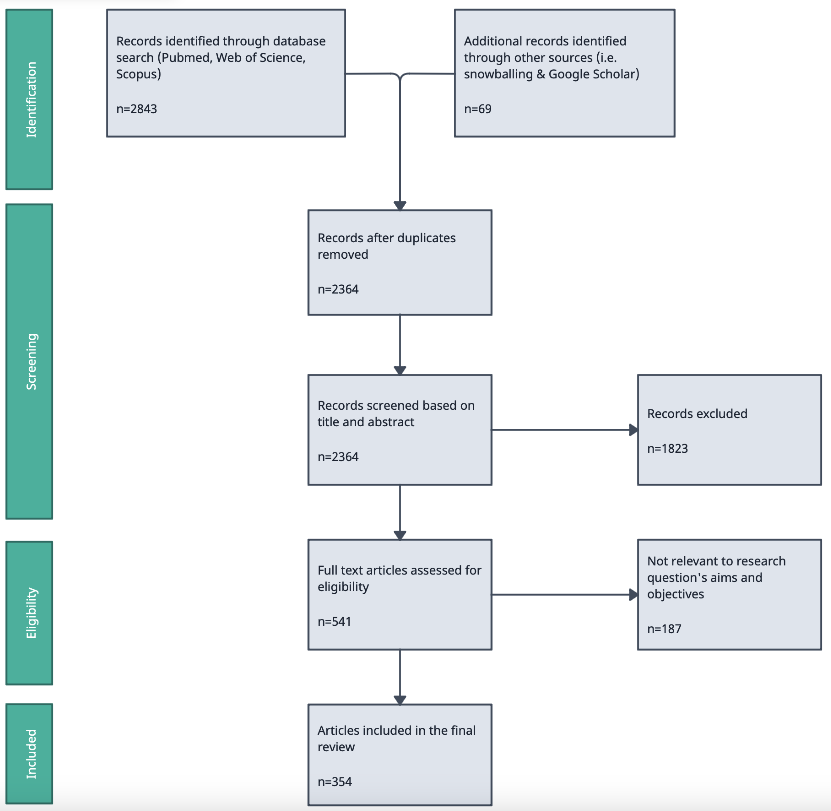
\includegraphics[keepaspectratio]{media/prisma.png}}
\end{column}
\end{columns}
\end{block}

\begin{block}{Literature search strategy II: Search string (Skip)}
\phantomsection\label{literature-search-strategy-ii-search-string-skip}
\begin{Shaded}
\begin{Highlighting}[]
\NormalTok{TITLE}\OperatorTok{{-}}\NormalTok{ABS}\OperatorTok{{-}}\NormalTok{KEY(}
\NormalTok{  (pandemic}\OperatorTok{*}\NormalTok{ OR epidemic}\OperatorTok{*}\NormalTok{ OR outbreak}\OperatorTok{*}\NormalTok{ OR }\StringTok{"public health crisis*"}\NormalTok{)}
\NormalTok{  AND}
\NormalTok{  (behavio}\OperatorTok{*}\NormalTok{r OR compliance OR adherence OR }\StringTok{"preventiv* measures"}\NormalTok{ OR }\StringTok{"protective measures"}\NormalTok{ OR mitigation OR }\StringTok{"health response*"} 
\NormalTok{    OR lockdown}\OperatorTok{*}\NormalTok{ OR }\StringTok{"stay at home"}\NormalTok{ OR }\StringTok{"social distan*"}\NormalTok{ OR quarantine OR }\StringTok{"mask* use"}\NormalTok{ OR }\StringTok{"mask wearing"}\NormalTok{ OR hygiene OR }\StringTok{"hand wash*"} 
\NormalTok{    OR }\StringTok{"vaccine acceptance"}\NormalTok{ OR }\StringTok{"vaccination intent*"}\NormalTok{ OR }\StringTok{"testing uptake"}\NormalTok{ OR }\StringTok{"contact tracing"}\NormalTok{ OR }\StringTok{"physical distancing"}\NormalTok{ OR }\StringTok{"non{-}pharmaceutical intervention*"}\NormalTok{)}
\NormalTok{)}
\NormalTok{AND}
\NormalTok{TITLE}\OperatorTok{{-}}\NormalTok{ABS}\OperatorTok{{-}}\NormalTok{KEY(}
\NormalTok{  (determinant}\OperatorTok{*}\NormalTok{ OR predictor}\OperatorTok{*}\NormalTok{ OR factor}\OperatorTok{*}\NormalTok{ OR driver}\OperatorTok{*}\NormalTok{ OR influenc}\OperatorTok{*}\NormalTok{)}
\NormalTok{  AND}
\NormalTok{  (economic OR }\StringTok{"socio{-}cultural"}\NormalTok{ OR social OR institutional OR psychological OR }\StringTok{"risk perception*"}\NormalTok{ OR cognitive OR affective OR normative }
\NormalTok{    OR }\StringTok{"peer effect*"}\NormalTok{ OR }\StringTok{"media influence*"}\NormalTok{ OR politic}\OperatorTok{*}\NormalTok{ OR demographic}\OperatorTok{*}\NormalTok{ OR cultural OR structural OR contextual)}
\NormalTok{)}
\end{Highlighting}
\end{Shaded}
\end{block}

\begin{block}{Social Cohesion \& Networks as determinants}
\phantomsection\label{social-cohesion-networks-as-determinants}
\begin{itemize}
\tightlist
\item
  \texttt{Peer\ Influence\ and\ Group\ Identity}

  \begin{itemize}
  \tightlist
  \item
    Individuals are more likely to adopt precautions (mask-wearing,
    distancing) when their immediate social networks and local
    influencers model these behaviors
    {[}20†L278-L286{]}{[}41†L649-L657{]}.
  \item
    Group identity reinforces compliance when health behaviors are seen
    as a mark of belonging
    {[}42†L157-L165{]}{[}45†L554-L562{]}{[}45†L574-L583{]}.
  \end{itemize}
\item
  \texttt{Community\ Trust\ \&\ Norms}

  \begin{itemize}
  \tightlist
  \item
    Tight-knit communities facilitate adherence to health measures
    {[}35†L165-L173{]}{[}51†L707-L715{]}.
  \item
    Partisan identities and in-group norms can override other favtors,
    leading to selective compliance or even counter-normative behavior
    {[}33†L167-L175{]}{[}33†L173-L180{]}.
  \end{itemize}
\end{itemize}
\end{block}

\begin{block}{Demographic Dynamics \& Knowledge}
\phantomsection\label{demographic-dynamics-knowledge}
\begin{itemize}
\tightlist
\item
  \texttt{Demographic\ Variations\ in\ Compliance}

  \begin{itemize}
  \tightlist
  \item
    Older adults, due to higher risk perception, tend to comply more
    with guidelines {[}22†L346-L354{]}{[}22†L347-L355{]}.
  \item
    Women exhibit higher compliance than men {[}25†L651-L658{]}.
  \item
    Higher education correlates with better understanding of COVID-19
    transmission and increased adherence {[}25†L649-L657{]}.
  \end{itemize}
\item
  \texttt{Economic\ and\ Informational\ Factors}

  \begin{itemize}
  \tightlist
  \item
    Lower-income groups often faced economic constraints that reduced
    their ability to comply {[}60†L161-L169{]}.
  \item
    Reliable knowledge from public health sources spurred early adoption
    of measures, whereas misinformation (\emph{infodemic}) undermined
    compliance {[}25†L659-L667{]}{[}28†L243-L251{]}.
  \end{itemize}
\end{itemize}
\end{block}

\begin{block}{Cultural Factors}
\phantomsection\label{cultural-factors}
\begin{itemize}
\tightlist
\item
  \texttt{Individualism\ vs.\ Collectivism}

  \begin{itemize}
  \tightlist
  \item
    Collectivist societies (e.g., many East Asian countries) achieved
    higher compliance by emphasizing group welfare, while
    individualistic cultures (e.g., the US, UK) often resisted
    restrictions {[}6†L141-L149{]}{[}6†L143-L151{]}.
  \end{itemize}
\item
  \texttt{Hierarchy\ and\ Norm\ Enforcement}

  \begin{itemize}
  \tightlist
  \item
    High power-distance cultures readily accepted top-down mandates
    {[}55†L840-L848{]}{[}55†L842-L846{]}
  \item
    Societies characterized by cultural tightness enforced uniform
    adherence through strict norms {[}20†L244-L252{]}{[}20†L254-L260{]}.
  \item
    Faith communities sometimes adapted rituals to support public health
    (as seen in Poland and Ghana) {[}18†L347-L355{]}{[}18†L351-L359{]}.
  \item
    Others resisted restrictions citing religious freedom
    {[}19†L315-L324{]}.
  \end{itemize}
\end{itemize}
\end{block}

\begin{block}{Gaps}
\phantomsection\label{gaps}
\begin{block}{LMICs}
\phantomsection\label{lmics}
\begin{itemize}
\tightlist
\item
  Mostly descriptive \& qualitative
\item
  Limited comparison of NPI vs Vaccines
\end{itemize}

\begin{block}{Dynamic interactions}
\phantomsection\label{dynamic-interactions}
\begin{itemize}
\tightlist
\item
  Factors mostly modelled in isolation
\item
  Crucial interactions sometimes assumed but never causally traced

  \begin{itemize}
  \tightlist
  \item
    Eg interaction of risk perceptions vs economic vulnerability
  \end{itemize}
\end{itemize}
\end{block}

\begin{block}{Cross border \& longitudinal comparisons}
\phantomsection\label{cross-border-longitudinal-comparisons}
\begin{itemize}
\tightlist
\item
  Almost exclusively single country, single time-period studies
\end{itemize}
\end{block}
\end{block}
\end{block}

\begin{block}{Aims \& research frameworks}
\phantomsection\label{aims-research-frameworks}
\begin{longtable}[]{@{}
  >{\raggedright\arraybackslash}p{(\linewidth - 2\tabcolsep) * \real{0.1515}}
  >{\raggedright\arraybackslash}p{(\linewidth - 2\tabcolsep) * \real{0.8485}}@{}}
\toprule\noalign{}
\begin{minipage}[b]{\linewidth}\raggedright
Chapter
\end{minipage} & \begin{minipage}[b]{\linewidth}\raggedright
Research question
\end{minipage} \\
\midrule\noalign{}
\endhead
\texttt{1} & What are the core mechanisms and interactions through which
economic, socio-cultural, institutional, and psychological determinants
shape individual compliance with public health measures during pandemics
in LMICs? \\
\texttt{2} & What is the causal impact of economic constraints relative
to health risk perceptions and vice versa on compliance with public
health measures in Malawi? \\
\texttt{3} & What is the causal effect of membership in non
self-selected peer groups on adherence to public health measures during
pandemics? \\
\bottomrule\noalign{}
\end{longtable}

\note{C1 \& C2: Both NPI and vaccines C3: NPI}
\end{block}
\end{frame}

\begin{frame}{Theoretical Frameworks that (don't) connect these factors}
\phantomsection\label{theoretical-frameworks-that-dont-connect-these-factors}
\begin{block}{Frameworks: Theory of plnned behaviour}
\phantomsection\label{frameworks-theory-of-plnned-behaviour}
\begin{figure}[H]

{\centering \pandocbounded{\includegraphics[keepaspectratio]{media/figure_1._theory_planned_behavior_model_adapted_from_ajzen_2005._456.webp}}

}

\caption{REFERENCE/SOURCE}

\end{figure}%
\end{block}

\begin{block}{Frameworks: Health Belief Model}
\phantomsection\label{frameworks-health-belief-model}
\begin{figure}[H]

{\centering \pandocbounded{\includegraphics[keepaspectratio]{media/Health_belief_model_diagram.jpg}}

}

\caption{REFERENCE/SOURCE}

\end{figure}%
\end{block}
\end{frame}

\begin{frame}[fragile]{Chapter I: Comparative structural modelling to
inform a theory of pandemic behaviour}
\phantomsection\label{chapter-i-comparative-structural-modelling-to-inform-a-theory-of-pandemic-behaviour}
RQ: What are the core mechanisms and interactions through which
economic, socio-cultural, institutional, and psychological determinants
shape individual compliance with public health measures during pandemics
in LMICs?

\begin{block}{Background \& Gaps}
\phantomsection\label{background-gaps}
\begin{columns}[T]
\begin{column}{0.48\linewidth}
\begin{itemize}
\tightlist
\item
  Some studies use theoretical frameworks (HBM \texttt{OR} TPB) to
  analyse survey data
\item
  Only REFERENCE in LMIC (Looking at students in Turkey)
\item
  No paper integrating/ extending these in C19 in LMIC
\item
  No study comparing different geographical contexts
\item
  No comparison of NPI and vaccines
\end{itemize}
\end{column}

\begin{column}{0.04\linewidth}
\end{column}

\begin{column}{0.48\linewidth}
\pandocbounded{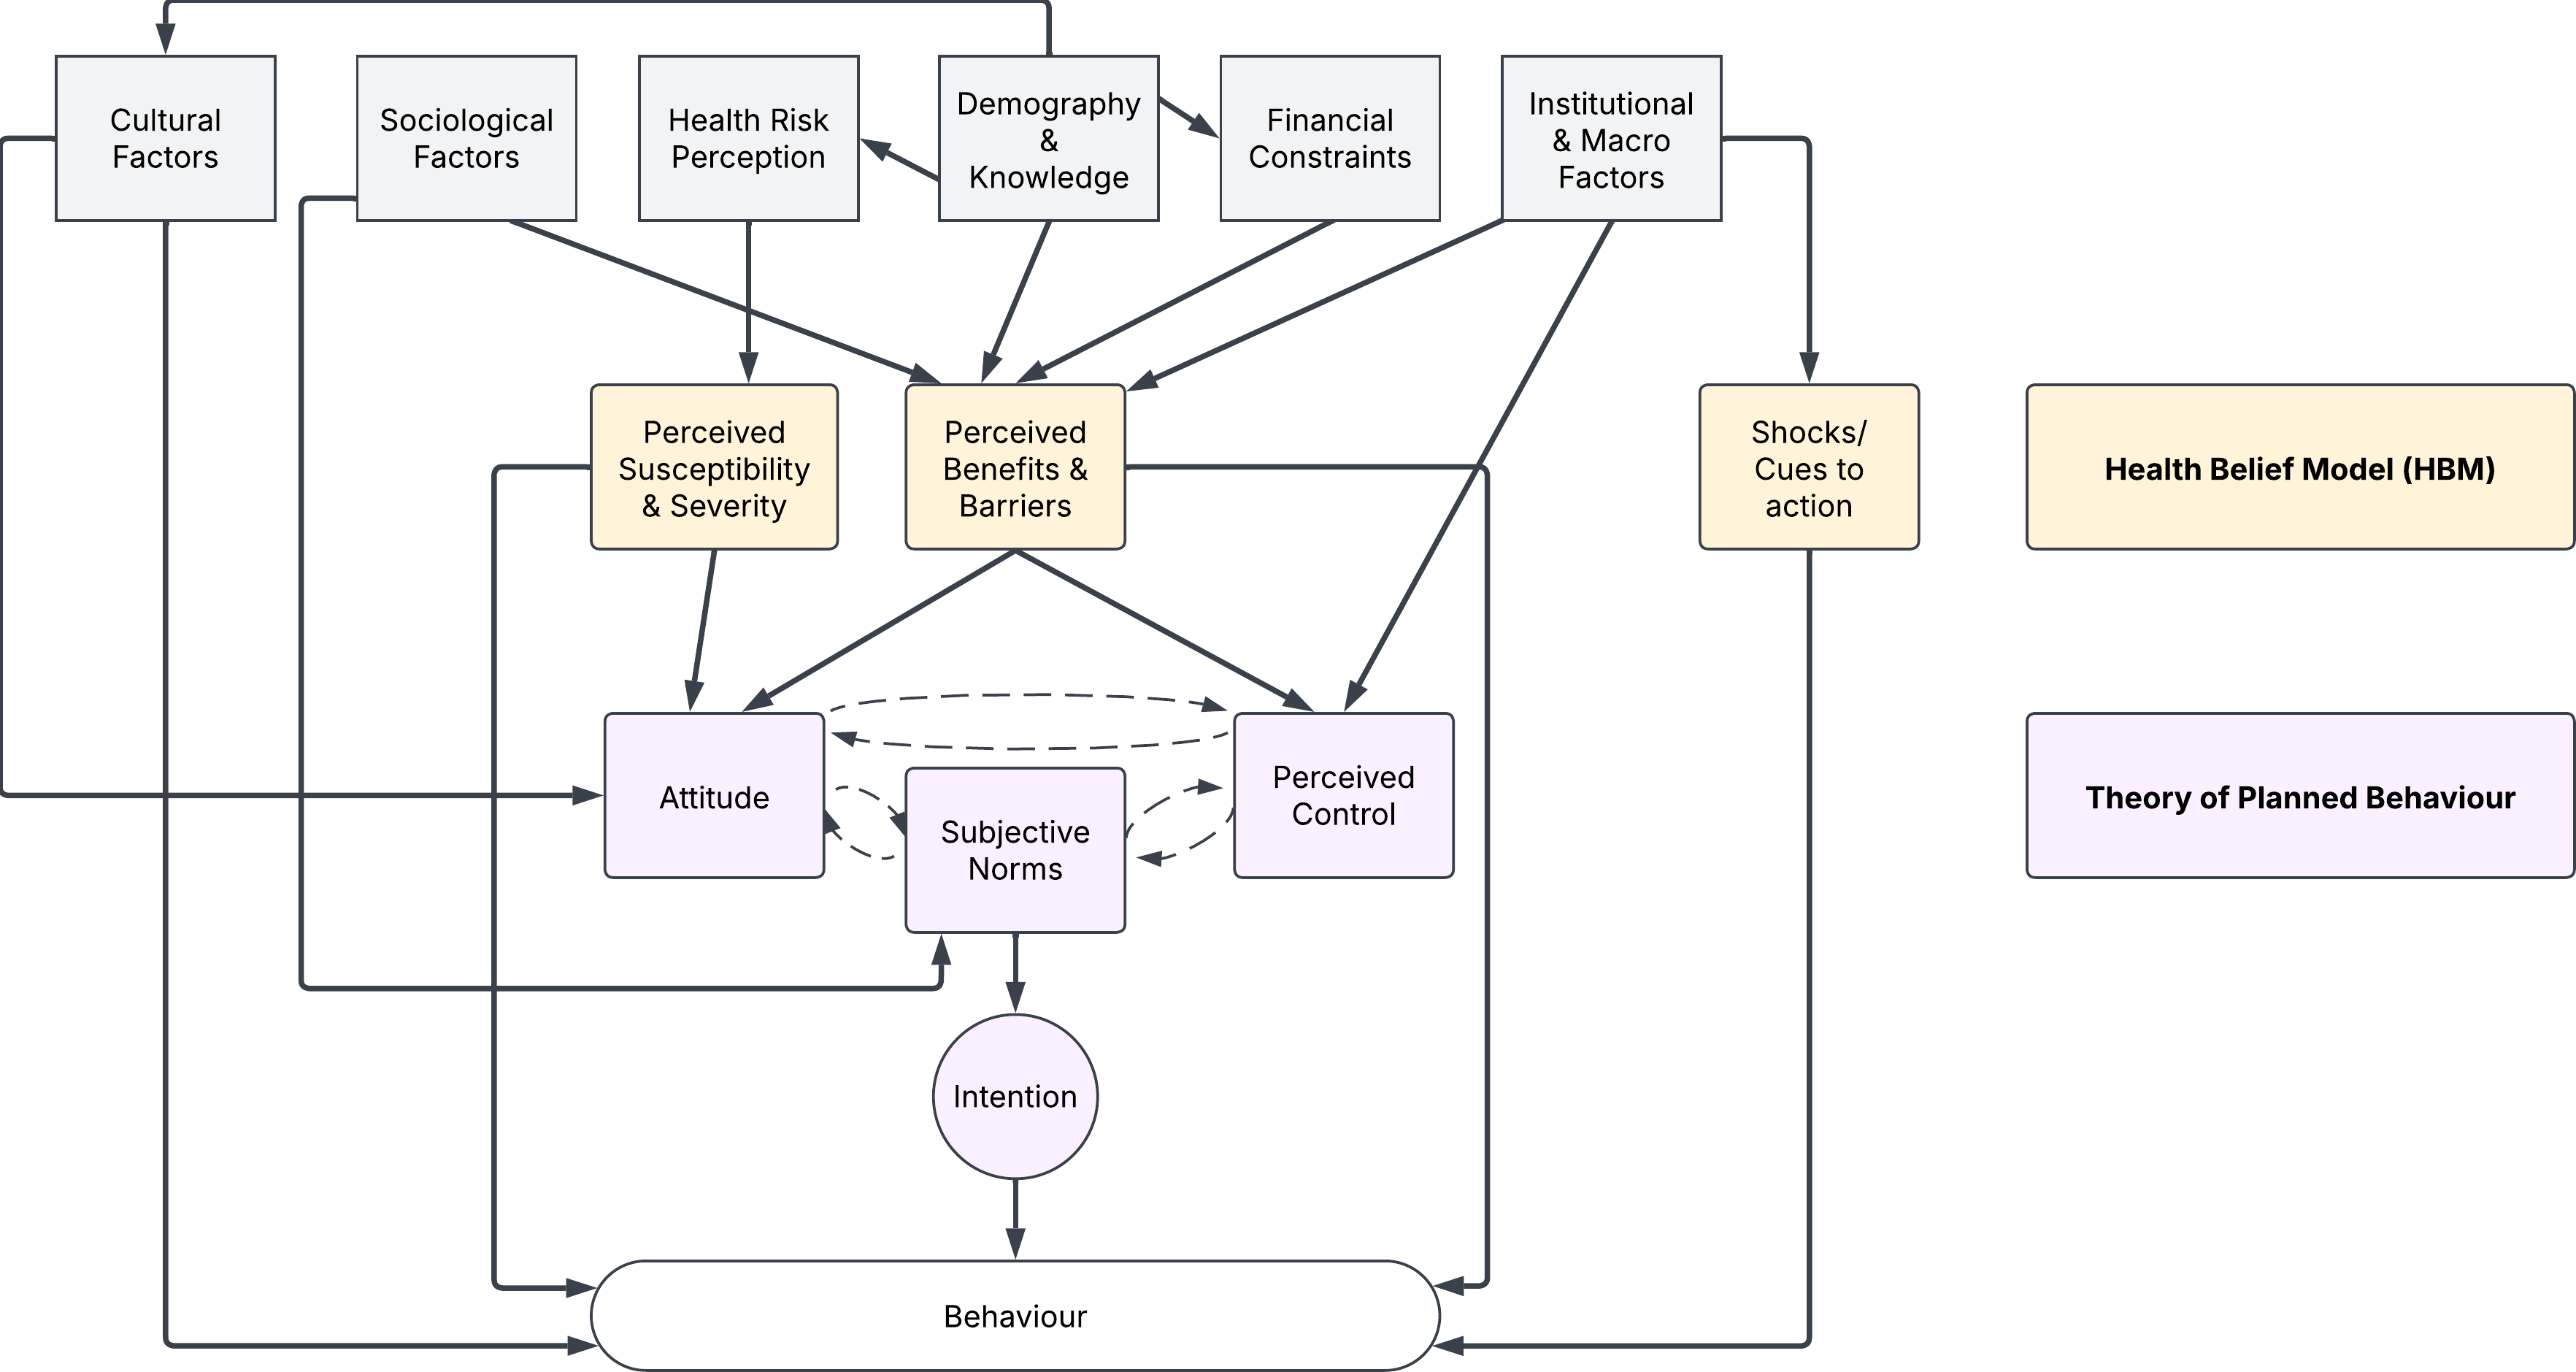
\includegraphics[keepaspectratio]{media/Screenshot 2025-03-04 at 21.02.23.png}}
\end{column}
\end{columns}
\end{block}

\begin{block}{Methods}
\phantomsection\label{methods}
\begin{block}{Approach}
\phantomsection\label{approach}
\begin{itemize}
\tightlist
\item
  Structural equation modelling to uncover latent and observed pathways

  \begin{itemize}
  \tightlist
  \item
    Allows simultaneous estimation of direct and indirect effects in
    predicting preventive behavior
  \end{itemize}
\item
  Direct, indirect, and total effects analysed for all models
\item
  Conducted at different waves for robustness checks and comparison
\end{itemize}
\end{block}
\end{block}

\begin{block}{Data}
\phantomsection\label{data}
\begin{block}{MIT C19 preventative health survey}
\phantomsection\label{mit-c19-preventative-health-survey}
\begin{itemize}
\tightlist
\item
  Conducted via online surveys distributed to Facebook users globally
\item
  Over 100k observations across 78 countries
\item
  Weighted to account for probability of being FB user
\item
  Contains data on all aforementioned factors
\item
  Repeated cross sectional survey
\end{itemize}
\end{block}
\end{block}

\begin{block}{Why: Contributions}
\phantomsection\label{why-contributions}
\begin{block}{Emprical contribution}
\phantomsection\label{emprical-contribution}
\begin{itemize}
\tightlist
\item
  First large scale SEM across countries and waves
\item
  Qunatification of uncertainity and relative importance of factors
\end{itemize}
\end{block}

\begin{block}{Theoretical Contribution}
\phantomsection\label{theoretical-contribution}
\begin{itemize}
\tightlist
\item
  Informing more comprehensive framework of pandemic behaviour
\item
  Introducing nuance around different intervention types (NPIs vs
  vaccine)
\end{itemize}
\end{block}

\begin{block}{Policy relevance}
\phantomsection\label{policy-relevance}
\begin{itemize}
\tightlist
\item
  Informs more efficient data collections during early phases of
  emergencies
\item
  Informs ressource allocation efficiency
\end{itemize}
\end{block}
\end{block}
\end{frame}

\begin{frame}[fragile]{Chapter II: Causally testing and qunatifying the
health-income trade-off assumption}
\phantomsection\label{chapter-ii-causally-testing-and-qunatifying-the-health-income-trade-off-assumption}
RQ: What is the causal impact of economic constraints relative to health
risk perceptions and vice versa on compliance with public health
measures in Malawi?

\begin{block}{Background \& Gaps}
\phantomsection\label{background-gaps-1}
\begin{block}{Widely assumed trade-off that \texttt{individuals} face}
\phantomsection\label{widely-assumed-trade-off-that-individuals-face}
\begin{itemize}
\tightlist
\item
  Rationale behind cash transfer programmes
\item
  Supported by economic theory (Grossman (19X); Prospect Theory)
\item
  Empirical eveidence shows

  \begin{itemize}
  \tightlist
  \item
    Effects of income
  \item
    Effects of risk perceptions
  \end{itemize}
\item
  Income and risk perception never modelled together to confirm
  \texttt{trade-off} in causal way
\end{itemize}
\end{block}
\end{block}

\begin{block}{Hypotheses}
\phantomsection\label{hypotheses}
\begin{block}{H1(2): Economic vulnerability (health risk perceptions)
predict compliance.}
\phantomsection\label{h12-economic-vulnerability-health-risk-perceptions-predict-compliance.}
\end{block}

\begin{block}{H3: Individuals face a trade-off between preserving their
health and their economic security.}
\phantomsection\label{h3-individuals-face-a-trade-off-between-preserving-their-health-and-their-economic-security.}
\end{block}
\end{block}

\begin{block}{Methods: Double Debiased Machine Learning}
\phantomsection\label{methods-double-debiased-machine-learning}
\begin{block}{Flexible ML to model covariate effect on treatment \&
outcome}
\phantomsection\label{flexible-ml-to-model-covariate-effect-on-treatment-outcome}
\begin{itemize}
\tightlist
\item
  Predict outcome/ treatment seperately given vector of covariates using
  ML methods
\end{itemize}
\end{block}

\begin{block}{Orthogonalised regression on residuals to estimate causal
effect of treatment and outcome}
\phantomsection\label{orthogonalised-regression-on-residuals-to-estimate-causal-effect-of-treatment-and-outcome}
\begin{itemize}
\tightlist
\item
  \emph{leftover variation of \texttt{treatemnt}} -\textgreater{}
  \emph{leftover variation of \texttt{outcome}}

  \begin{itemize}
  \tightlist
  \item
    Given no OVB
  \end{itemize}
\item
  Based on Neyman (19XX)
\end{itemize}
\end{block}
\end{block}

\begin{block}{Data}
\phantomsection\label{data-1}
\begin{block}{World Bank Malawi high frequency phone survey between 2020
and 2024}
\phantomsection\label{world-bank-malawi-high-frequency-phone-survey-between-2020-and-2024}
\begin{itemize}
\tightlist
\item
  Subset: 05/20-07/21

  \begin{itemize}
  \tightlist
  \item
    Only the first 13 rounds contain information about
    non-pharmaceutical mitigation behaviour
  \end{itemize}
\item
  Nationally representative sample of households based on the Malawi
  National Integrated Household Panel Survey from 2019
\item
  1729 participants at baseline \& 8\% attrition at R13
\item
  Further weighting based on census data
\end{itemize}
\end{block}
\end{block}

\begin{block}{Why: Contributions}
\phantomsection\label{why-contributions-1}
\begin{block}{Emprical contribution}
\phantomsection\label{emprical-contribution-1}
\begin{itemize}
\tightlist
\item
  First causal investigation into health/income trade-off in context of
  protective measures during a pandemic
\item
  Qunatification of trade-off and comparison over time
\end{itemize}
\end{block}

\begin{block}{Theoretical Contribution}
\phantomsection\label{theoretical-contribution-1}
\begin{itemize}
\tightlist
\item
  Empirical test of widely-assumed trade-off assumption
\end{itemize}
\end{block}

\begin{block}{Policy relevance}
\phantomsection\label{policy-relevance-1}
\begin{itemize}
\tightlist
\item
  Informs more efficient data collections during early phases of
  emergencies
\item
  Informs ressource allocation efficiency
\end{itemize}
\end{block}
\end{block}
\end{frame}

\begin{frame}{Chapter: Peer effects vs self selection}
\phantomsection\label{chapter-peer-effects-vs-self-selection}
RQ: What is the causal effect of membership in non self-selected peer
groups on adherence to public health measures during pandemics?

\begin{block}{Background \& Gaps}
\phantomsection\label{background-gaps-2}
\end{block}

\begin{block}{Methods}
\phantomsection\label{methods-1}
\end{block}

\begin{block}{Data}
\phantomsection\label{data-2}
\end{block}

\begin{block}{Why: Contributions}
\phantomsection\label{why-contributions-2}
\begin{block}{Emprical contribution}
\phantomsection\label{emprical-contribution-2}
\end{block}

\begin{block}{Theoretical Contribution}
\phantomsection\label{theoretical-contribution-2}
\end{block}

\begin{block}{Policy relevance}
\phantomsection\label{policy-relevance-2}
\end{block}
\end{block}
\end{frame}

\begin{frame}{Thank you!}
\phantomsection\label{thank-you}
\end{frame}

\begin{frame}{Questions \& Feedback}
\phantomsection\label{questions-feedback}
\end{frame}

\begin{frame}{Annex I: Chapter I}
\phantomsection\label{annex-i-chapter-i}
\begin{block}{Annex: Structural Equation Modelling II (Skip)}
\phantomsection\label{annex-structural-equation-modelling-ii-skip}
\begin{block}{Confirmatory Factor Analysis (CFA)}
\phantomsection\label{confirmatory-factor-analysis-cfa}
\begin{itemize}
\tightlist
\item
  To validate latent constructs
\item
  To operationalise constructs from survey items
\end{itemize}
\end{block}

\begin{block}{Comparative Model Evaluation}
\phantomsection\label{comparative-model-evaluation}
\begin{itemize}
\tightlist
\item
  Predictive power assessment (variance explained in preventative
  behavior)
\item
  Multi-group SEM for cross-country/SES/gender comparisons
\item
  Akaike Information Criterion (AIC) \& Bayesian Information Criterion
  (BIC) for model comparison
\end{itemize}
\end{block}
\end{block}
\end{frame}

\begin{frame}[fragile]{Annex II Chapter 2}
\phantomsection\label{annex-ii-chapter-2}
\begin{block}{Annex: Chapter II BG: Malawi during waves 1 \& 2 of C19}
\phantomsection\label{annex-chapter-ii-bg-malawi-during-waves-1-2-of-c19}
\pandocbounded{\includegraphics[keepaspectratio]{media/Malawitimeline.png}}
\end{block}

\begin{block}{Annex: Chapter II How: Outcomes}
\phantomsection\label{annex-chapter-ii-how-outcomes}
\begin{longtable}[]{@{}
  >{\raggedright\arraybackslash}p{(\linewidth - 6\tabcolsep) * \real{0.2075}}
  >{\raggedright\arraybackslash}p{(\linewidth - 6\tabcolsep) * \real{0.4528}}
  >{\raggedright\arraybackslash}p{(\linewidth - 6\tabcolsep) * \real{0.1698}}
  >{\raggedright\arraybackslash}p{(\linewidth - 6\tabcolsep) * \real{0.1698}}@{}}
\toprule\noalign{}
\begin{minipage}[b]{\linewidth}\raggedright
\texttt{Outcome}
\end{minipage} & \begin{minipage}[b]{\linewidth}\raggedright
Indicators
\end{minipage} & \begin{minipage}[b]{\linewidth}\raggedright
Investigation at
\end{minipage} & \begin{minipage}[b]{\linewidth}\raggedright
Hypothesis tests
\end{minipage} \\
\midrule\noalign{}
\endhead
\textbf{\texttt{Social\ distancing}} & Gathering attendance;
non-essential travels; Reduced Shopping & Multiple rounds & H1, H2,
H3 \\
\textbf{\texttt{Hygiene\ \&\ Mask}} & Hand Washing; Mask Wearing &
Single Round & H2 \\
\textbf{\texttt{Willingness\ to\ test}}* & Willingness to test & Single
Round & H1 \\
\textbf{\texttt{Vaccine\ Acceptance*}} & Willingness to vaccinate &
Single round & H1 \\
\bottomrule\noalign{}
\end{longtable}

*Vaccines and tests are provided for free but involve significant
transaction and opportunity costs. Reddy, K.P., Fitzmaurice, K.P.,
Scott, J.A. et al.~Clinical outcomes and cost-effectiveness of COVID-19
vaccination in South Africa. Nat Commun 12, 6238 (2021)
\end{block}

\begin{block}{Annex: Chapter II How: Treatments I}
\phantomsection\label{annex-chapter-ii-how-treatments-i}
\begin{block}{Economic Vulnerability Indicator}
\phantomsection\label{economic-vulnerability-indicator}
\begin{itemize}
\tightlist
\item
  Constructed from factors such as:

  \begin{itemize}
  \tightlist
  \item
    Current income
  \item
    Self-reported economic stability perception
  \item
    Economic risk perception due to the pandemic
  \item
    Main income source (formal vs.~informal economy)
  \item
    Consumption quantile (based on monthly spending)
  \end{itemize}
\item
  Operationalization methods under consideration:

  \begin{itemize}
  \tightlist
  \item
    Inverse Probability Weighting (IPW) by Anderson
  \item
    Established economic vulnerability measures (e.g., Calvo \& Dercon,
    2005)
  \item
    Data-driven approach (PCA or single factor analysis)
  \end{itemize}
\end{itemize}
\end{block}
\end{block}

\begin{block}{Annex: Chapter II How: Treatments II}
\phantomsection\label{annex-chapter-ii-how-treatments-ii}
\begin{block}{Health Risk Perception Indicator}
\phantomsection\label{health-risk-perception-indicator}
\begin{itemize}
\tightlist
\item
  Self-reported health risk perception
\item
  Infection history and self-reported comorbidities
\item
  Recent Covid-19 symptoms
\end{itemize}
\end{block}

\begin{block}{Trade-off as interaction term}
\phantomsection\label{trade-off-as-interaction-term}
\end{block}
\end{block}

\begin{block}{Annex: Chapter II How: Controlling for \ldots{}}
\phantomsection\label{annex-chapter-ii-how-controlling-for}
\begin{itemize}
\tightlist
\item
  Demographics (Age, gender, education, urban/rural, etc.)
\item
  Cultural affiliations and beliefs (religion, parties, norms, etc.)
\item
  HH characteristics (size, adult equiv., etc.)
\item
  Exposure to C19
\item
  Trust in institutions \& conspiracy beliefs
\item
  Mental health
\item
  Macro context (policies, economic performance, etc.)
\item
  And some more (self-efficacy, C19 communication exposure, news
  consumption, etc.)
\end{itemize}
\end{block}

\begin{block}{Annex: Chapter II How: Challenges of traditional
econometric approaches I}
\phantomsection\label{annex-chapter-ii-how-challenges-of-traditional-econometric-approaches-i}
\pandocbounded{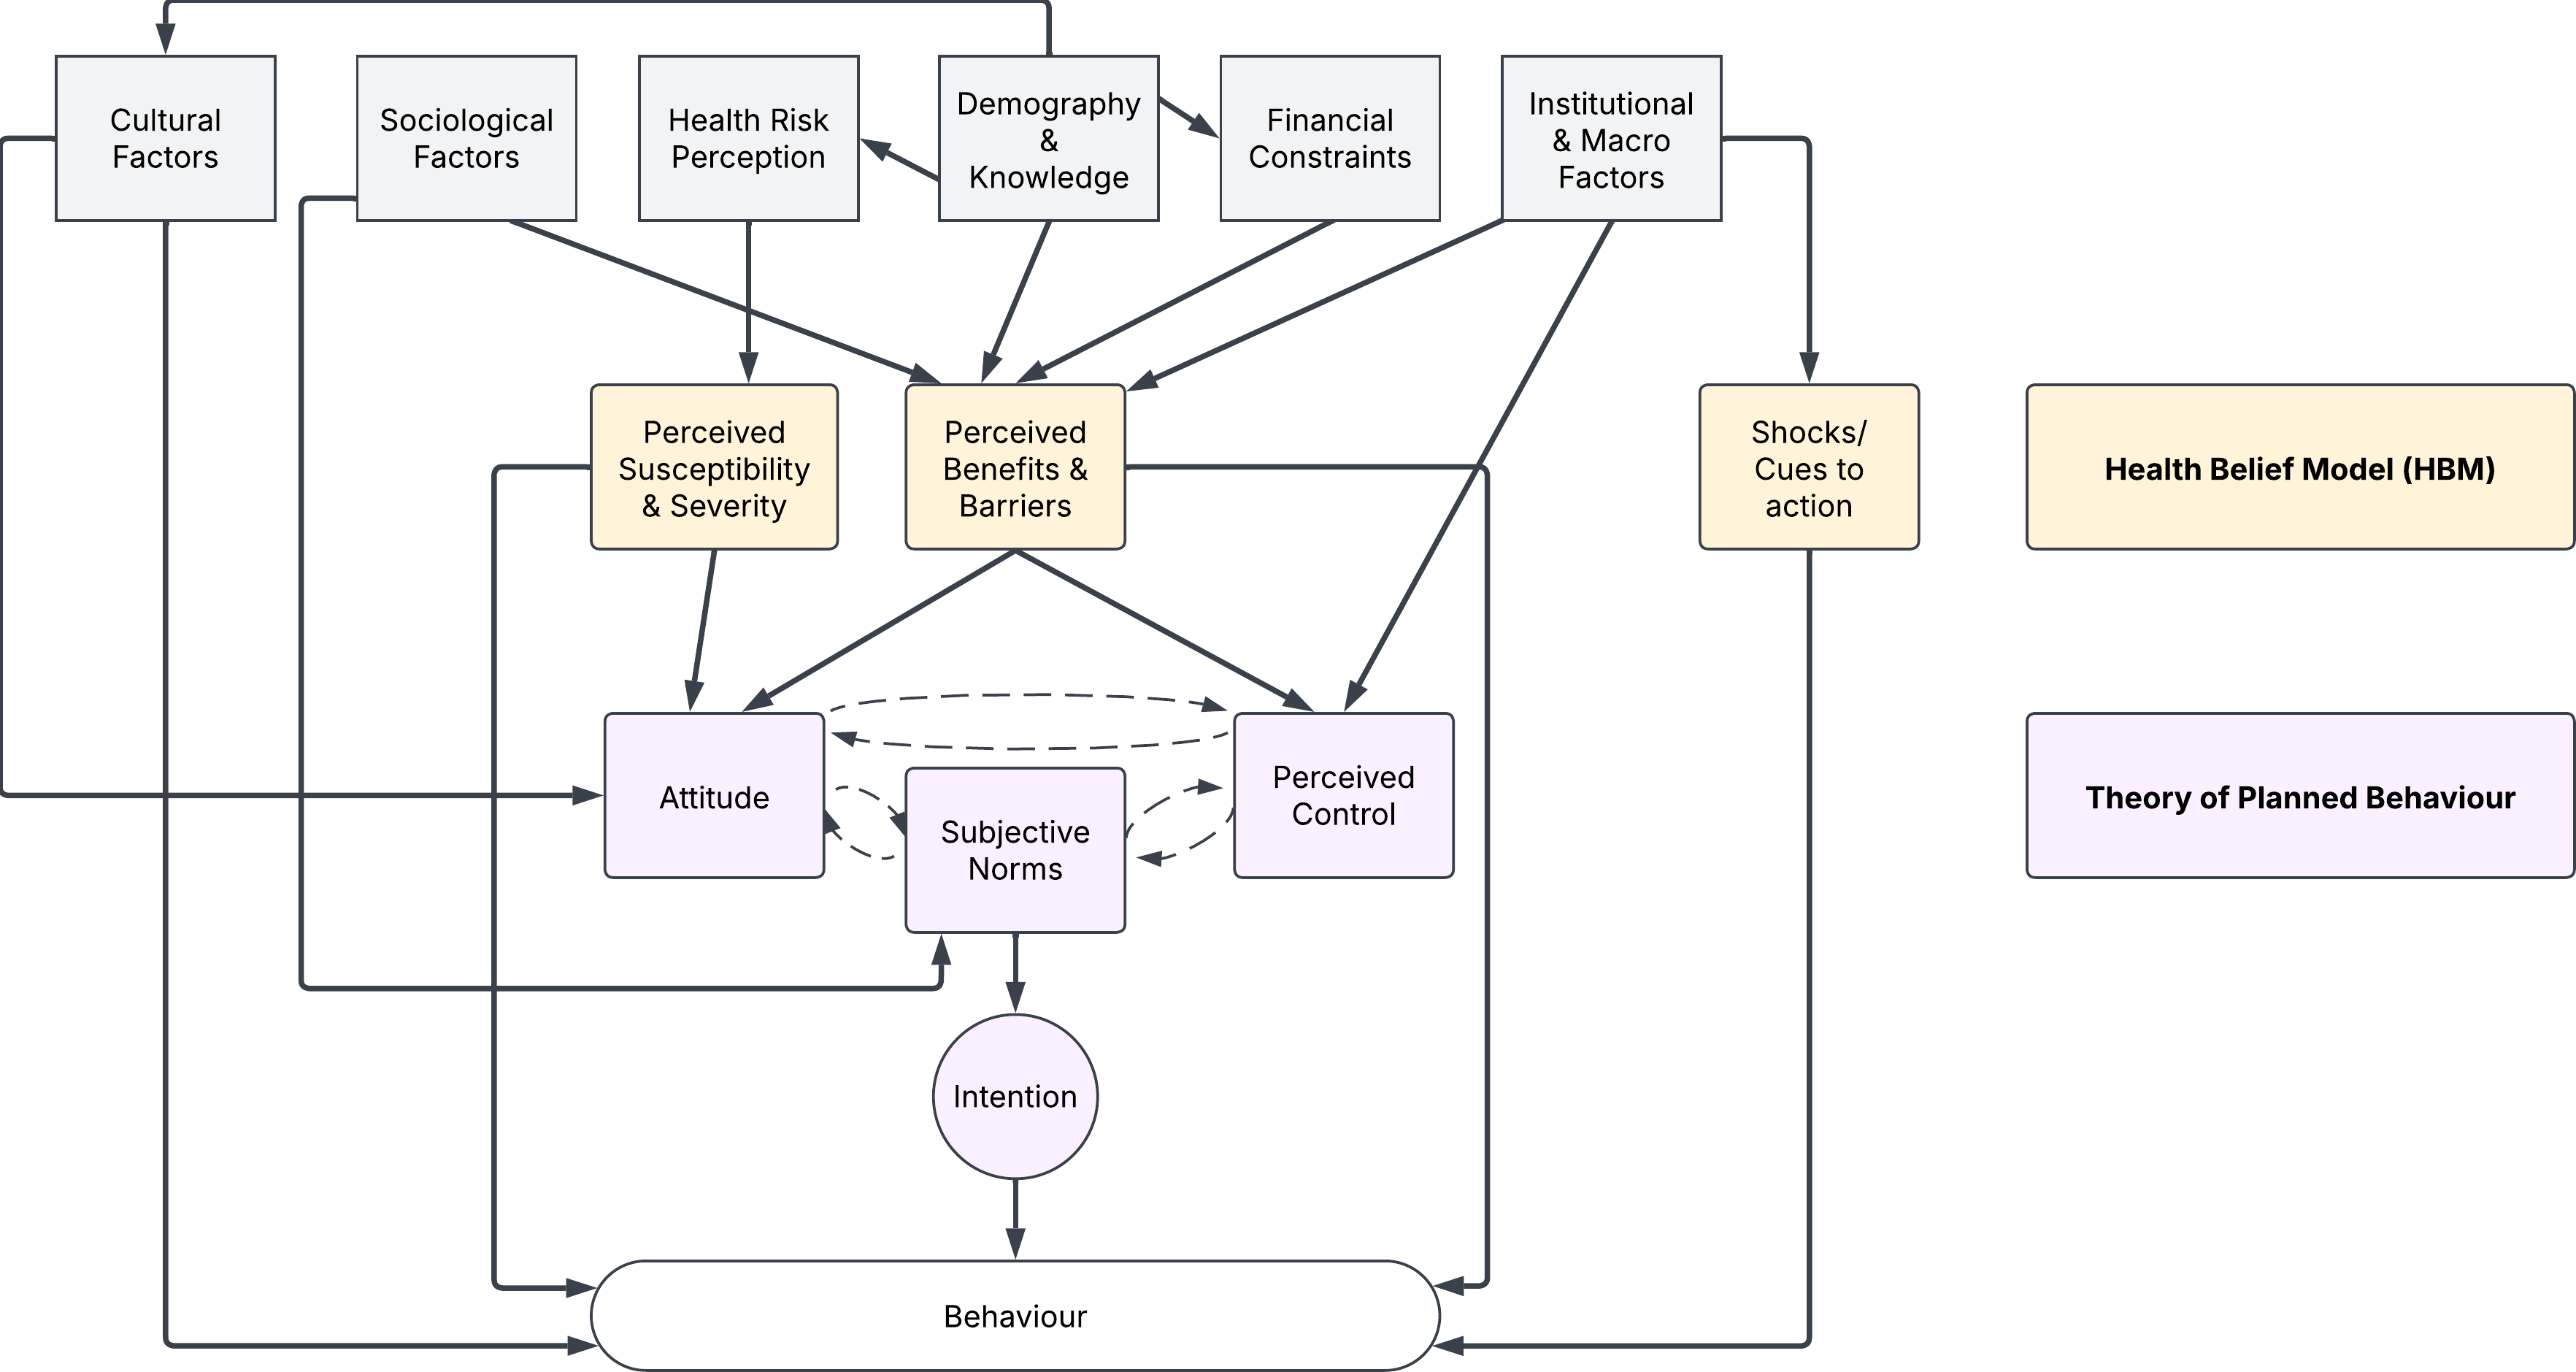
\includegraphics[keepaspectratio]{media/Screenshot 2025-03-04 at 21.02.23.png}}
\end{block}

\begin{block}{Annex: Chapter II How: Challenges of traditional
econometric approaches II}
\phantomsection\label{annex-chapter-ii-how-challenges-of-traditional-econometric-approaches-ii}
\begin{block}{Strengths}
\phantomsection\label{strengths}
\begin{itemize}
\tightlist
\item
  Interpretability
\item
  Causal pathway identification
\end{itemize}
\end{block}

\begin{block}{Limitations}
\phantomsection\label{limitations}
\begin{itemize}
\tightlist
\item
  Exogeneity concerns

  \begin{itemize}
  \tightlist
  \item
    Either RCT or
  \item
    Quasiexperimental approach difficult with income
  \item
    Controlling requires many functional assumptions
  \end{itemize}
\end{itemize}
\end{block}
\end{block}

\begin{block}{Annex: Chapter II How: Challenges of machine learning}
\phantomsection\label{annex-chapter-ii-how-challenges-of-machine-learning}
\begin{block}{Strengths}
\phantomsection\label{strengths-1}
\begin{itemize}
\tightlist
\item
  Very flexible re functional forms
\item
  Can handle large amounts of covariates
\end{itemize}
\end{block}

\begin{block}{Limitations}
\phantomsection\label{limitations-1}
\begin{itemize}
\tightlist
\item
  Overfitting concerns
\item
  Causal pathway interpretation challenging
\end{itemize}
\end{block}
\end{block}

\begin{block}{Annex: Chapter II How: Double Debiased Machine Learning
II}
\phantomsection\label{annex-chapter-ii-how-double-debiased-machine-learning-ii}
\begin{block}{Cross-fitting to reduce overfitting and regularization
bias}
\phantomsection\label{cross-fitting-to-reduce-overfitting-and-regularization-bias}
\pandocbounded{\includegraphics[keepaspectratio]{media/dmlcrossfit.png}}
\end{block}
\end{block}
\end{frame}

\begin{frame}{Annex III Chapter 3}
\phantomsection\label{annex-iii-chapter-3}
\end{frame}




\end{document}
